\section{Zielsetzung}
\label{sec:Zielsetzung}
\nocite{anleitungV203}
Das Ziel des Versuchs ist die Verdampfungswärme $L$ von Wasser zu ermitteln. Hierfür wird Wasser erhitzt und
die Temperatur sowie der Dampfdruck gemessen.

\section{Theorie}
\label{sec:Theorie}
Wasser kann in drei verschiedenen Phasen bzw. Aggregatzuständen fest, flüssig und gasförmig vorliegen.
Diese Zustände sind von dem Druck $p$ und der Temperatur $T$ abhängig. In der Abbildung (\ref{fig:ZustandsdiagrammWasser})
ist die Temperatur- sowie die Druckabhängigkeit des Wasserzustands qualitativ abgebildet.
\begin{figure}[H]
    \centering
    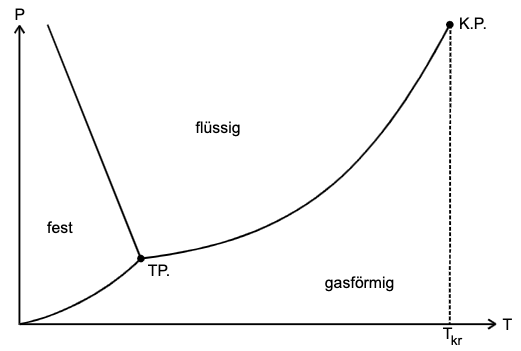
\includegraphics[width=0.90\textwidth]{ZustandsdiagrammWasser.png}
    \caption{Qualitatives Zustandsdiagramm von Wasser. \cite{anleitungV203}}
    \label{fig:ZustandsdiagrammWasser}
\end{figure}
Innerhalb der drei abgeschlossenen Bereichen, welche den drei genannten Phasen von Wasser entsprechen, besitzt das System 
zwei Freiheitsgrade $p$ und $T$. Dahingegen besitzt das System nur einen Freiheitsgrad, wenn sich den Grenzlinien angenähert wird. An diesen
Grenzlinien koexistieren zwei Phasen. Am Tripelpunkt (TP.) befindet sich das Wasser im festen, flüssigen als auch im gasförmigen Zustand.
An dem kritischen Punkt koexisiteren die flüssige und gasförmige Phase. 
Die Grenzlinie, die den Tripelpunkt und den kritischen Punkt verbindet, wird Dampfdruckkurve genannt. Dabei wird die Dampfdruckkurve
durch die molare Verdampfungswärme $L$ charakterisiert. Diese Größe beschreibt die Energie, welche notwendig ist, um bestimmte Stoffmengen
zu verdampfen. Im allgemeinen ist die Verdampfungswärme $L$ stoff- und temperaturabhängig. Allerdings ist $L$ im Bereich der Messung bis zu $1\,\unit{\bar}$  
nahezu temperaturunabhängig und wird daher als konstant angenommen. Die Verdampfungswärme $L$ ergibt sich aus der inneren Verdampfungswärme $L_{\text{i}}$
und der äußeren Verdampfungswärme $L_{\text{a}}$. Somit ergibt sich 
\begin{equation}
    L = L_{\text{i}} + L_{\text{a}}\,.
    \label{eqn:Verdampfungswaerme}
\end{equation}
$L_{\text{i}}$ beschreibt die Arbeit zur Überwindung der molekularen Anziehungskräfte und $L_{\text{a}}$ ist die Energie, die benötigt wird, um das Volumen eines Stoffes vor der Verdampfung $V_{\text{F}}$
auf das Volumen eines Stoffes nach der Verdampfung $V_{\text{D}}$ auszudehnen.
Dieser Vorgang ist anschaulich in der Abbildung (\ref{fig:Kreisprozess}) dargestellt. Hier wird der Verdampfungs- und Kondensationsprozess eines Stoffes in Abhängigkeit vom Druck $p$ und des Volumens $V$
betrachtet.
\begin{figure}[H]
    \centering
    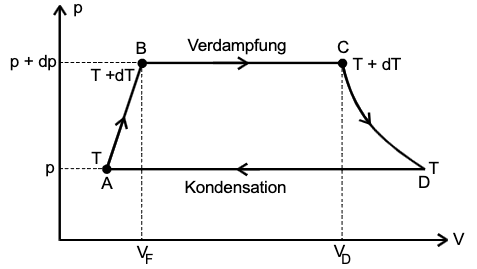
\includegraphics[width=0.95\textwidth]{Kreisprozess.png}
    \caption{Kreisprozess eines Stoffes in einem p-V-Diagramm. \cite{anleitungV203}}
    \label{fig:Kreisprozess}
\end{figure}
Mithilfe des Kreisprozesses in Abbildung (\ref{fig:Kreisprozess}) lässt sich die Clausius-Clapeyronsche Gleichung
\begin{equation}
    \left(V_{\text{D}} - V_{\text{F}}\right)\text{dp} = \frac{L}{T}\,\text{d}T
    \label{eqn:ClausiusClapeyronscheGleichung}
\end{equation}
bestimmen. Mit dieser Gleichung wird der Verlauf der Dampfdruckkurve eines Stoffes charakterisiert. Wird eine Temperatur betrachtet, welche deutlich kleiner als
der kritische Temperatur $T_{\text{Kr}}$ ist, werden mehrere Annahmen getroffen. Zunächst wird angenommen, dass $V_{\text{F}}$ deutlich kleiner als $V_{\text{D}}$ ist und somit
$V_{\text{F}}$ gegenüber $V_{\text{D}}$ vernachlässigbar ist. Demnach gilt für $V_{\text{D}}$ die ideale Gasgleichung 
\begin{equation}
    p \cdot V = R \cdot T\,.
    \label{eqn:idealeGasgleichung}
\end{equation}
Dabei ist $p$ der Druck, $V$ das Volumen, $R$ die allgemeine Gaskonstante und $T$ die Temperatur. Daher ergibt sich für die ideale Gasgleichung für $V_{\text{D}}$ 
\begin{equation}
    V_{\text{D}} \left(p,\, T\right) = R\cdot \frac{T}{p}
    \label{eqn:idealeGasgleichung_V_D}
\end{equation}
Wie bereits erwähnt, wird zudem $L$ als konstant betrachtet. Somit hängt $L$ nicht von dem Druck $p$ und der Temperatur $T$ ab. Daraus folgt durch
Integration der Gleichung (\ref{eqn:ClausiusClapeyronscheGleichung})
\begin{equation}
    p = p_{0} \cdot \exp{\left(-\frac{L}{R}\cdot \frac{1}{T}\right)}\,.
    \label{eqn:Druck_p}
\end{equation}
Diese Gleichung beschreibt nun den Verlauf der Dampfdruckkurve.
% \subsection{Vorbereitungsaufgaben}
% \label{sec:Vorbereitungsaufgaben}
